\documentclass[aspectratio=169]{beamer}
\usepackage[T1]{fontenc} \usepackage{lmodern} \usepackage[utf8]{inputenc}
\usepackage[english]{babel} \usepackage{booktabs}
\usepackage{graphicx,subcaption} \usepackage{amssymb,amsmath}
\graphicspath{{figures/}}
\usepackage[citestyle=authoryear,bibstyle=authoryear,backend=biber,url=false,doi=false,isbn=false]{biblatex} \bibliography{refs}
\usepackage{hyperref}

%------------------------------------------------

% https://hartwork.org/beamer-theme-matrix/
% http://www.cpt.univ-mrs.fr/~masson/latex/Beamer-appearance-cheat-sheet.pdf

% Sans-serif is easier to read. Keep for text.
% Math is nicer in serif, and easier to discriminate from text.
% But then it's inconsistent...
%\usefonttheme{serif}
\usefonttheme[onlymath]{serif}

\usetheme{Malmoe}
\setbeamertemplate{footline}[page number]
\setbeamertemplate{navigation symbols}{}

\definecolor{darkred}{rgb}{0.8,0,0}  % defined in beaver
\usecolortheme{beaver}
\setbeamercolor{structure}{fg=darkred,bg=white}
\setbeamercolor{block title}{fg=darkred,bg=white}

%------------------------------------------------

\newcommand{\HRule}{{\usebeamercolor[bg]{subsection in head/foot} \rule{\linewidth}{0.5mm}}}

%------------------------------------------------

\begin{document}

\begin{frame}[plain]
	%\titlepage
	\begin{center}

		\begin{minipage}{0.7\linewidth}
			\textsc{\large A Network Tour of Data Science}
		\end{minipage}
		\hfill
		\begin{minipage}{0.2\linewidth}
			\includegraphics[width=\linewidth]{logo_epfl}
		\end{minipage}
		\vspace{0.5cm}

		\HRule
		\vspace{0.55cm}
		{
			\usebeamercolor[fg]{frametitle}
			\textsc{\Large Projects}\\
			\vspace{0.3cm}
		}
		\HRule
		\vspace{0.8cm}

		\hspace{0.3cm}
		\begin{minipage}[t]{0.35\linewidth}
			\footnotesize
			\textbf{Teachers} \\
			Pierre \textsc{Vandergheynst} \\
			Pascal \textsc{Frossard} \\
			Andreas \textsc{Loukas} \\
			Michaël \textsc{Defferrard} \\
			Volodymyr \textsc{Miz} \\
		\end{minipage}
		\begin{minipage}[t]{0.25\linewidth}
			\footnotesize
			\textbf{Assistants} \\
			Michaël \textsc{Defferrard} \\
			Volodymyr \textsc{Miz} \\
			Effrosyni \textsc{Simou} \\
			Eda \textsc{Bayram} \\
		\end{minipage}
		\begin{minipage}[t]{0.25\linewidth}
			\footnotesize
			Benjamin \textsc{Ricaud} \\
			Nicolas \textsc{Aspert} \\
			Clément \textsc{Vignac} \\
			Guillermo \textsc{Jimenez} \\
			Nikolaos \textsc{Karalias} \\
		\end{minipage}

		\vspace{0.4cm}
		{\footnotesize EPFL LTS2 \& LTS4 laboratories
		\hfill November 6, 2019}

	\end{center}
\end{frame}

%------------------------------------------------

\begin{frame}
	\frametitle{Goal}
	\begin{center}
		\huge
		Tell a {\color{darkred}\textbf{data story}} or build a {\color{darkred}\textbf{data product}}.
	\end{center}
\end{frame}
% * Use the data to answer a research question you are curious about.
% * Use the data to build a ``product'', e.g., predict some variables given others.

%------------------------------------------------

\begin{frame}
	%\frametitle{Flow}
	%\frametitle{Process}
	\frametitle{How}
	% Explicit those points in the following slides.
	\begin{enumerate}
		\item Define a problem.
		\vfill
		\color{lightgray}
		\item Tackle it.
			\vspace{1em}
			\begin{itemize}
				\color{lightgray}
				\item Choose appropriate data and tools.
				\vspace{1em}
				\item Use the Data Science process and the scientific method.
				% (observations -> hypothesis -> experiments)
			\end{itemize}
		\vfill
		\item Communicate the results.
	\end{enumerate}
\end{frame}

%------------------------------------------------

\begin{frame}
	\frametitle{Example problems}
	% Should fall in both story and product category.
	\begin{description}
		\item[IMDb] How do actors choose a film to play in? Do they form communities? What are the characteristics of those communities?
		\vfill
		\item[FMA] Can an online music platform recommend annotations (such as tags or genres) to artists regarding their newly uploaded songs?
		\vfill
		\item[Senators] Are senators truly divided in republicans and democrats? Can I predict the votes of a senator knowing the votes of ``similar'' senators?
	\end{description}
	\vfill
	More ideas on GitHub. Come up with your own!
\end{frame}

%------------------------------------------------

\begin{frame}
	%\frametitle{Flow}
	%\frametitle{Process}
	\frametitle{How}
	% Explicit those points in the following slides.
	\begin{enumerate}
		\item {\color{lightgray} Define a problem.}
		\vfill
		\item Tackle it.
			\vspace{1em}
			\begin{itemize}
				\item Choose appropriate data and tools.
				\vspace{1em}
				\item Use the Data Science process and the scientific method.
				% (observations -> hypothesis -> experiments)
			\end{itemize}
		\vfill
		\color{lightgray}
		\item Communicate the results.
	\end{enumerate}
\end{frame}

%------------------------------------------------

% \begin{frame}
% 	\frametitle{Data and tools}
% 	list from github
% 	tools from the lecture slides
% \end{frame}

%------------------------------------------------

\begin{frame}
	\frametitle{Data science process}
	% If you remember the data science process
	\begin{figure}
		\includegraphics[height=0.85\textheight]{data_science_process}
	\end{figure}
\end{frame}

%------------------------------------------------

\begin{frame}
	%\frametitle{Flow}
	%\frametitle{Process}
	\frametitle{How}
	% Explicit those points in the following slides.
	\begin{enumerate}
		\item {\color{lightgray} Define a problem.}
		\vfill
		\item {\color{lightgray} Tackle it.}
			\vspace{1em}
			\begin{itemize}
				\color{lightgray}
				\item Choose appropriate data and tools.
				\vspace{1em}
				\item Use the Data Science process and the scientific method.
			\end{itemize}
		\vfill
		\item Communicate the results.
	\end{enumerate}
\end{frame}

%------------------------------------------------

\begin{frame}
	\frametitle{Communication}
	\begin{minipage}[t]{0.45\linewidth}
		\begin{figure}
			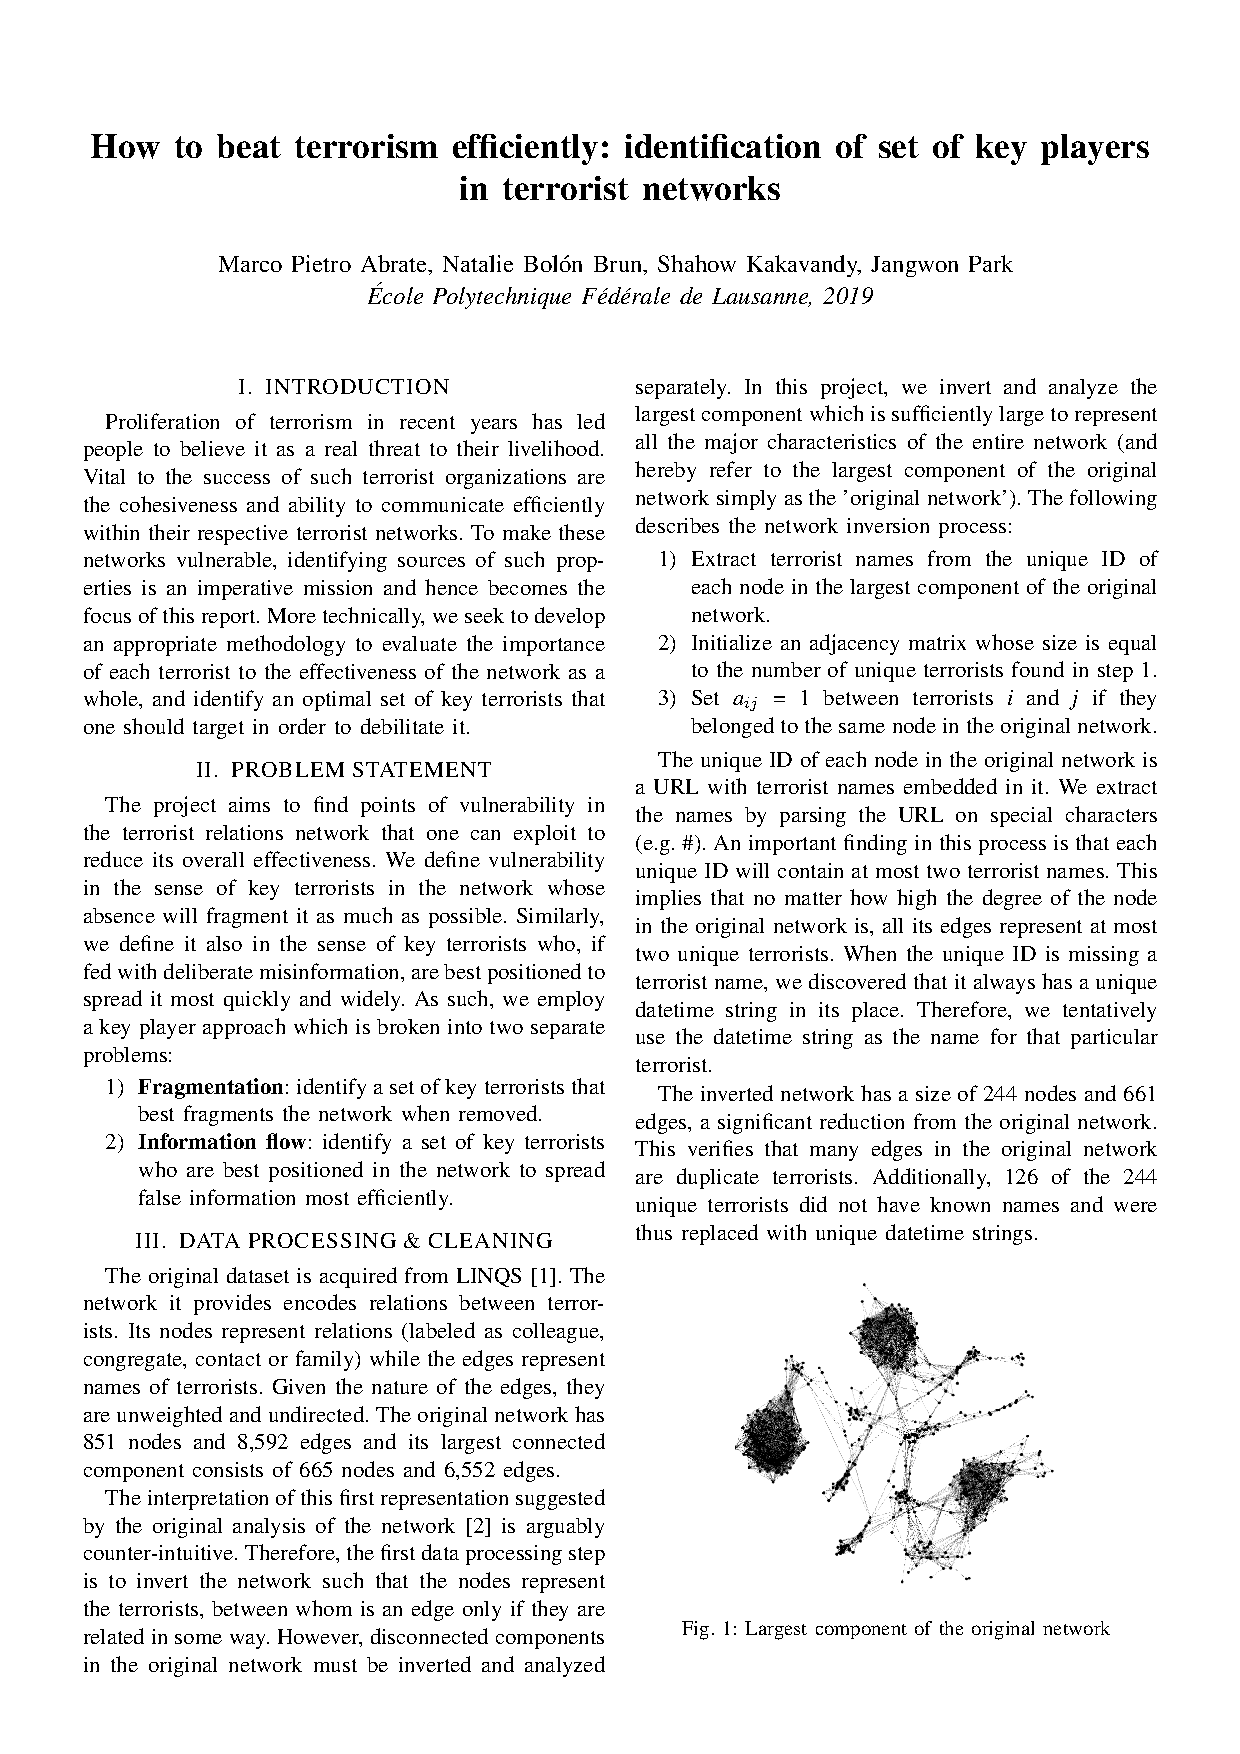
\includegraphics[width=\linewidth,trim={0 20cm 0 2cm},clip]{project_27_report}
			\caption*{\color{darkred} report}
		\end{figure}
		\vspace{-1em}
		\begin{figure}
			
\includegraphics[width=\linewidth,trim={0 0 0 7cm},clip]{project_27_slides}
			\caption*{\color{darkred} presentation}
		\end{figure}
	\end{minipage}
	\hfill
	\begin{minipage}[t]{0.45\linewidth}
		\begin{figure}
			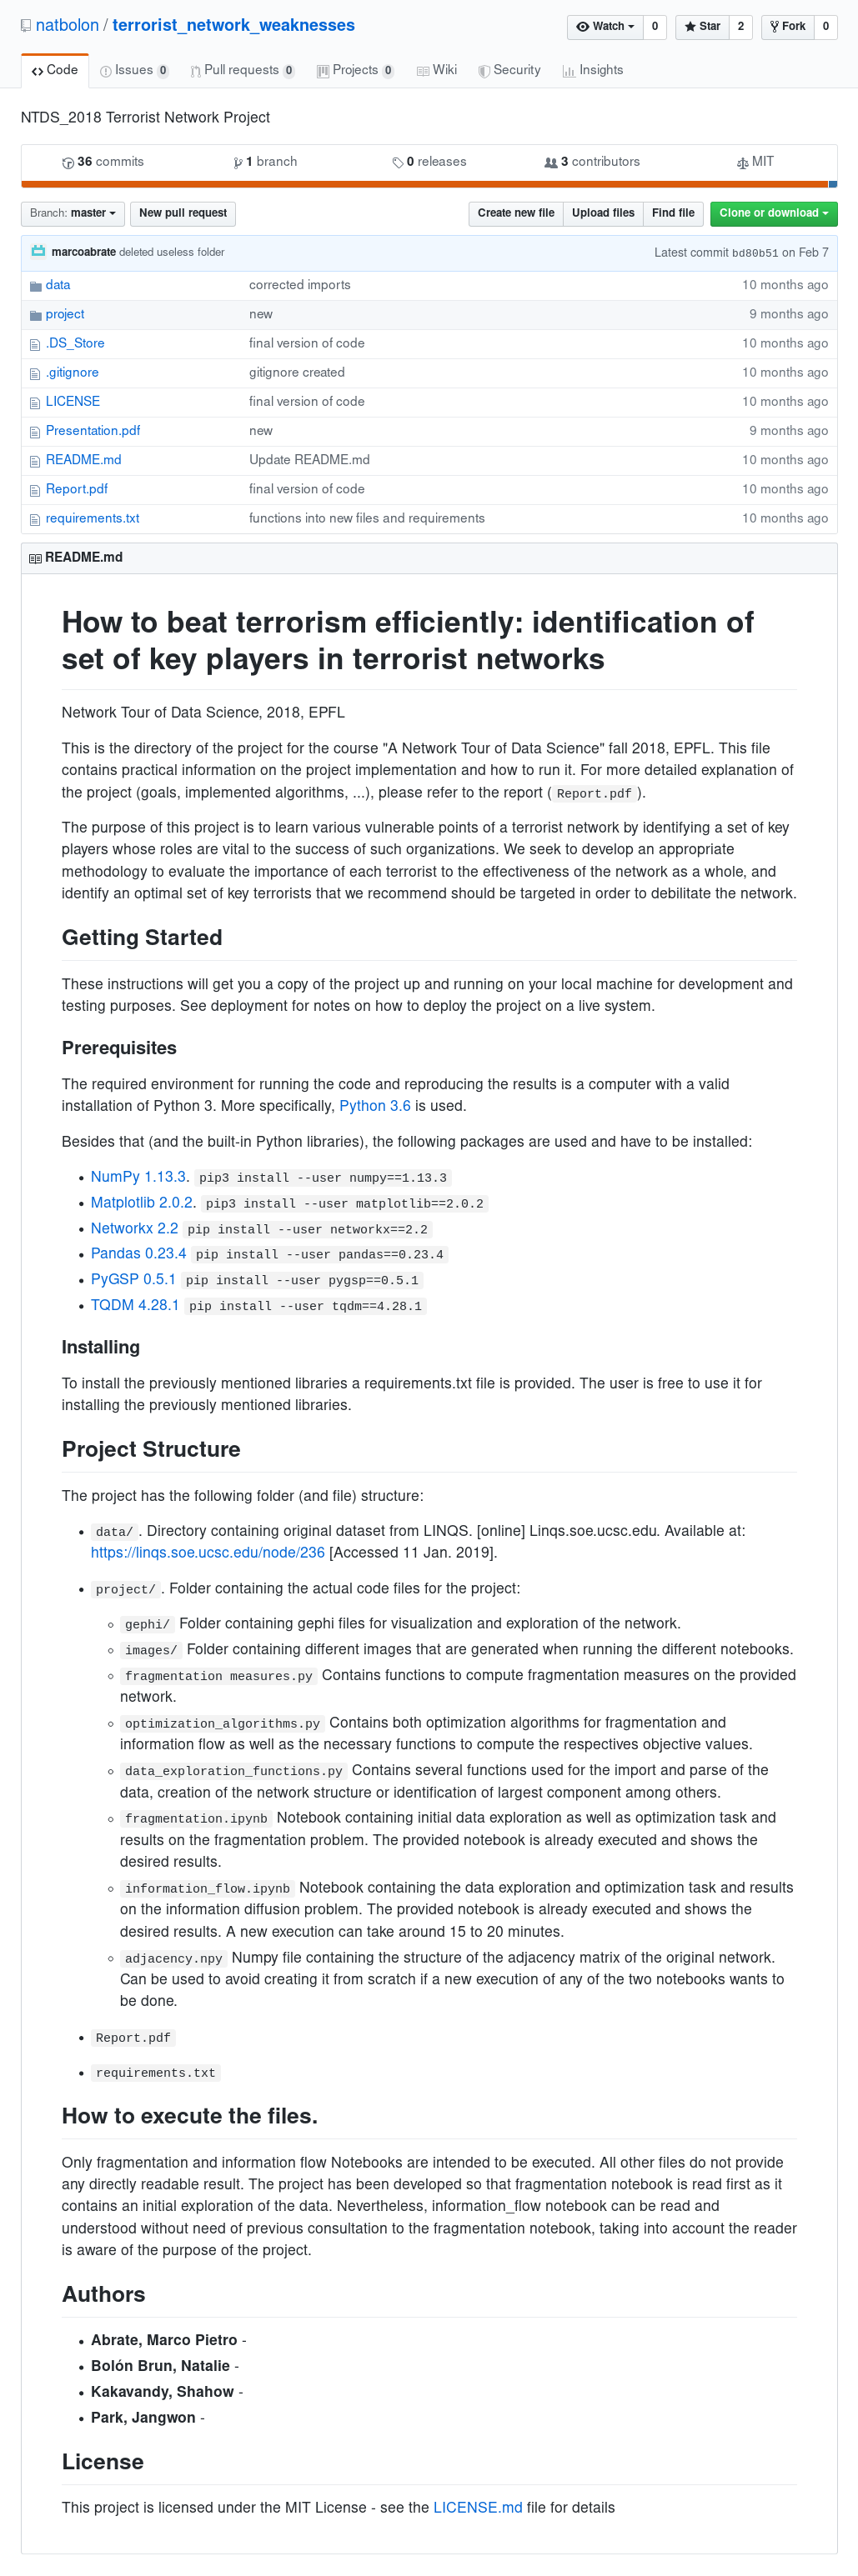
\includegraphics[width=\linewidth,trim={0 17.3cm 0 0},clip]{project_27_github}
			\caption*{\color{darkred} code repository}
		\end{figure}
	\end{minipage}
\end{frame}

%------------------------------------------------

\begin{frame}
	\frametitle{Beware}
	\begin{itemize}
		\item Set a goal that is attainable given your understanding of the data and tools.
		\vfill
		\item A project is not a set of experiments. It should be motivated and follow a story.
		\vfill
		\item Projects should use tools and ideas from the lectures. They should include graph and network data aspects, and more generally fall under the scope of the class.
		\vfill
		\item Building a good graph is as important as analyzing it. Your graph should be built towards the goal of solving your problem. %That includes sub-sampling.
	\end{itemize}
\end{frame}

%------------------------------------------------

\begin{frame}
	\frametitle{Grading criteria}
	\framesubtitle{Details on GitHub}
	\begin{enumerate}
		\item Story (20 points): motivation and choices
		\vfill
		\item Acquisition (10 points): getting data
		\vfill
		\item Exploration (20 points): understanding the data
		\vfill
		\item Exploitation (30 points): using the data
		\vfill
		\item Communication (20 points): communicating the results
	\end{enumerate}
\end{frame}

%------------------------------------------------

\begin{frame}
	\frametitle{Peer-review}
	A pedagogical tool to:
	\vfill
	\begin{enumerate}
		\item Receive feedback on your work.
		\vfill
		\item Understand the grading criteria. % by practicing them
	\end{enumerate}
	\vfill
\end{frame}

%------------------------------------------------

\begin{frame}
	\frametitle{Deliverables (intermediate peer-review)}
	\begin{description}
		\item[summary] Summarize your project. Four students will read it to evaluate your project. This evaluation won't count towards the project grade. The summary is a PDF of at most 1 page of text (and 1 supplementary page for figures and tables).
		\vfill
		\item[peer-review] Each student individually evaluates a project on the 5 grading criteria. The evaluation must be motivated. The motivations will be graded (10\% of the course grade).
	\end{description}
\end{frame}

%------------------------------------------------

\begin{frame}
	\frametitle{Deliverables (final evaluation)}
	\begin{description}
		\item [report] Describe your motivations, explain what you did and why, and state your conclusions. The report is a PDF of at most 5 pages.
		\vfill
		\item [code] All the code you developed for the project must be stored in a GitHub repository. It should contain a useful readme and a license. Code should be organized and clean.
		\vfill
		\item [presentation] Impress us! Presentations are 12 minutes long, followed by 3 minutes of questions. Each group member must talk.
	\end{description}
\end{frame}

%------------------------------------------------

\begin{frame}
	\frametitle{Deadlines}
	\begin{description}
		\item[Dec 4] submit the project summary
		\vfill
		\item[Dec 10] submit the peer-review report (individual)
		\vfill
		\item[Jan 10] submit the project report
		\vfill
		\item[Jan 10] submit a link to the project's GitHub repository
		\vfill
		\item[Jan 21-22] give an oral presentation
		\vfill
		\item[Jan 24] upload the presentation slides
	\end{description}
\end{frame}

%------------------------------------------------

\begin{frame}
	\frametitle{Resources}
	\href{https://github.com/mdeff/ntds_2019}{GitHub}:
	\begin{itemize}
		\vspace{0.5em}
		\item Dataset and project ideas
		\vspace{0.5em}
		\item Grading criteria
	\end{itemize}
	\vfill
	Past projects:
	\begin{itemize}
		\vspace{0.5em}
		\item NTDS'18: \url{https://github.com/mdeff/ntds_2018}
		\vspace{0.5em}
		\item NTDS'17: \url{https://github.com/mdeff/ntds_2017}
	\end{itemize}
\end{frame}

%------------------------------------------------

\begin{frame}
	\begin{figure}
		\centering
		\includegraphics[trim={0 19.9cm 0 0},clip,width=\linewidth]{projects_2018}
	\end{figure}
	\begin{center}
		\Huge Have fun!
		\hspace{2em}
		\Huge Questions?
	\end{center}
	\begin{figure}
		\centering
		\includegraphics[trim={0 0 0 19.9cm},clip,width=\linewidth]{projects_2018}
	\end{figure}
\end{frame}

%------------------------------------------------

\end{document}
